\section{Theoretische Grundlagen}
\label{sec:grundlagen}
Zu Beginn werden die theoretischen Grundlagen betrachtet, die eine Basis für das Verständnis der vorliegenden Ausarbeitung darstellen.
	\subsection{Wärmeübertragung}
	\label{sec:waermeuebertragung}
Die Wärmeübertragung beschreibt die gegenseitigen Abhängigkeiten von Temperaturfeldern und Wärmeströmen \cite{Langeheinecke2008}. Es gibt drei Arten, wie Wärme übertragen werden kann:
\begin{itemize}
	\item Wärmeleitung
	\item Wärmekonvektion
	\item Wärmestrahlung
\end{itemize}
Die \textbf{Wärmeleitung} beschreibt die Übertragung von Wärme innerhalb eines Körpers. Die Größe des Wärmestromes hängt von dem vorliegenden Temperaturgradienten und Material ab. Die Kenngröße des Materials ist die Wärmeleitfähigkeit $\lambda \left[\frac{W}{m*K}\right]$. Allgemein gilt für die Wärmeleitung das \textit{Gesetz von Fourier} nach Gleichung \ref{eq:gesetz-von-fourier}, wobei r eine Ortskoordinate ist \cite{Boeckh2015}.
\begin{equation}
	\label{eq:gesetz-von-fourier}
	\dot{q} \left[\frac{W}{m²}\right]=-\lambda*\frac{d\vartheta}{dr} 
\end{equation}

Bla bla bla. Hier noch ein Bild zur Veranschaulichung:

\begin{figure}[h]
	\centering
	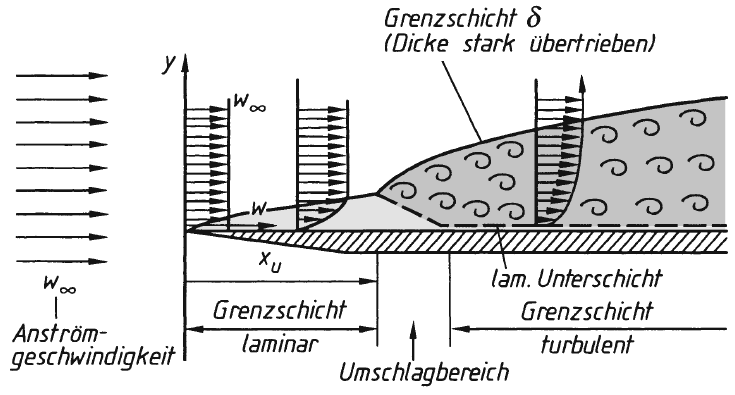
\includegraphics[width=0.7\textwidth]{Bilder/grenzschichttheorie}
	\caption{Veranschaulichung der Grenzschichttheorie \cite{Boeswirth2014}}
	\label{img:grenzschichttheorie}
\end{figure}

Und hier noch eine Referenz zur Einleitung, siehe Kapitel \ref{sec:einleitung}.\\
Danach noch eine Tabelle als Beispiel.\\

Im folgenden Abschnitt sollen die chemischen Reaktionen untersucht werden, die zu Ablagerungsprodukten führen. Die wichtigen festen Folgeprodukte der Harnstoffzersetzung sind in Tabelle \ref{tbl:harnstofffolgeprodukte} gelistet.

	\nomenclature[cBIU]{NH\textsubscript{2}-CO-NH-CO-NH\textsubscript{2}}{Biuret}
	\nomenclature[cTRIU]{NH\textsubscript{2}-CO-NH-CO-NH-CO-NH\textsubscript{2}}{Triuret}
	\nomenclature[cCYA]{C\textsubscript{3}N\textsubscript{3}(OH)\textsubscript{3}}{Cyanursäure}
	\nomenclature[cAMELID]{C\textsubscript{3}N\textsubscript{3}(OH)\textsubscript{2}NH\textsubscript{2}}{Ammelid}
	\nomenclature[cAMELIN]{C\textsubscript{3}N\textsubscript{3}OH(NH\textsubscript{2})\textsubscript{2}}{Ammelin}
	\nomenclature[cMEL]{C\textsubscript{3}N\textsubscript{3}(NH\textsubscript{2})\textsubscript{3}}{Melamin}

\begin{table}[h]
	\centering
	\begin{tabular}{C{2,2 cm}|C{5,4 cm}|C{2,8 cm}|C{2,8 cm}}
		\centering \textbf{Produkt} &
		\centering \textbf{chemische Formel} &
		\centering \textbf{Schmelzpunkt} &
		\centering \textbf{Zersetzungs-beginn}\tabularnewline
		\hline
		Biuret & NH\textsubscript{2}-CO-NH-CO-NH\textsubscript{2} & 193\,°C & 193\,°C\\
		Triuret & NH\textsubscript{2}-CO-NH-CO-NH-CO-NH\textsubscript{2} & 231\,°C & ca. 220\,°C\\
		Cyanursäure & C\textsubscript{3}N\textsubscript{3}(OH)\textsubscript{3} & 320\,°C - 330\,°C & ca. 220\,°C\\
		Ammelid & C\textsubscript{3}N\textsubscript{3}(OH)\textsubscript{2}NH\textsubscript{2} &  & 270\,°C\\
		Ammelin & C\textsubscript{3}N\textsubscript{3}OH(NH\textsubscript{2})\textsubscript{2} &  & 300\,°C\\
		Melamin & C\textsubscript{3}N\textsubscript{3}(NH\textsubscript{2})\textsubscript{3} & 354\,°C - 357\,°C & 354\,°C - 357\,°C\\
		
	\end{tabular}
	\caption{Wichtige Folgeprodukte der Harnstoffzersetzung, chemische Formeln und charakteristische Temperaturen, zusammengestellt aus \cite{Brack2016}.}
	\label{tbl:harnstofffolgeprodukte}
\end{table}
 

	\nomenclature[i0]{0}{normiert}
	\nomenclature[rW]{$w$}{Tangentialgeschwindigkeit $\left[\frac{m}{s}\right]$}
	\nomenclature[rR]{$R$,$r$}{Radius [m]}
	\nomenclature[cSTICKSTOFFMO]{NO}{Stickstoffmonoxid}	
	\nomenclature[cSTICKSTOFFDI]{NO\textsubscript{2}}{Stickstoffdioxid}
	\nomenclature[cAMMONIAK]{NH\textsubscript{3}}{Ammoniak}
	\nomenclature[cKOHLENMONO]{CO}{Kohlenstoffmonoxid}
	\nomenclature[cKOHLENDIO]{CO\textsubscript{2}}{Kohlenstoffdioxid}
	\nomenclature[rT]{$T$}{Temperatur [K]}
	\nomenclature[rC]{$c$}{Schallgeschwindigkeit $\left[\frac{m}{s}\right]$}
	\nomenclature[rM1]{$M$}{molare Masse $\left[\frac{g}{mol}\right]$}
	\nomenclature[rN]{$n$}{Stoffmenge [mol]}
	\nomenclature[rM3]{$\dot m$}{Massenstrom $\left[\frac{kg}{h}\right]$}
	\nomenclature[rNPUNKT]{$\dot n$}{molarer Strom $\left[\frac{mol}{h}\right]$}
	\nomenclature[rL]{$L$}{charakteristische Länge [m]}
	\nomenclature[gl]{$\alpha$}{Wärmeübergangskoeffizient $\left[\frac{W}{m²*K}\right]$}
	\nomenclature[iFl]{Fl}{Fluid}
	\nomenclature[iW]{W}{Wand}
	\nomenclature[iMSCR]{mSCR}{modulare SCR-Strecke}
	\nomenclature[rNu]{\textit{Nu}}{Nusselt-Zahl [-]}
	\nomenclature[rr]{$r$}{Ortskoordinate [m]}
	\nomenclature[gt]{$\vartheta$}{Temperatur [°C]}
	\nomenclature[gl]{$\lambda$}{Wärmeleitkoeffizient $\left[\frac{W}{m*K}\right]$}
	\nomenclature[rQPUNKTk]{$\dot q$}{spezifischer Wärmestrom $\left[\frac{W}{m²}\right]$}
